\graphicspath{{chapters/chapter7/imgs/}}

\chapter{Wyniki}\label{chapter:ch7}

Gitara siema byczku

\section{Demografia}\label{section:ch7_1}

W badaniu wzięły udział 34 osoby, gdzie 14 uczestników wypełniło formularz A, a 20 osób formularz B.
Rozkład płci uczestników był stosunkowo wyrównany - w przypadku formularza A, 8 osób to kobiety, 4 to
mężczyźni, a 2 nie podały płci. Z kolei wśród wypełniających formularz B, 7 osób to kobiety, 12 to
mężczyźni, a 1 osoba wybrała opcję "Inna" w pytaniu o płeć. Te informacje można odczytać z tabeli \ref{tab1:ch7_1}
i rysunku \ref{fig:ch7_demo1} .

\begin{table}[h!]
    \begin{center}
        \begin{tabular}{|l|r|r|}
            \hline
            Płeć      & Liczba osób & Procent całości \\
            \hline
            Kobieta   & 16          & 47.06\%         \\
            Mężczyzna & 17          & 50.00\%         \\
            Inne      & 1           & 2.94\%          \\
            \hline
        \end{tabular}
    \end{center}
    \caption{Uczestnicy badania ze względu na płeć}\label{tab1:ch7_1}
\end{table}

\begin{figure}[h!]
    \centering
    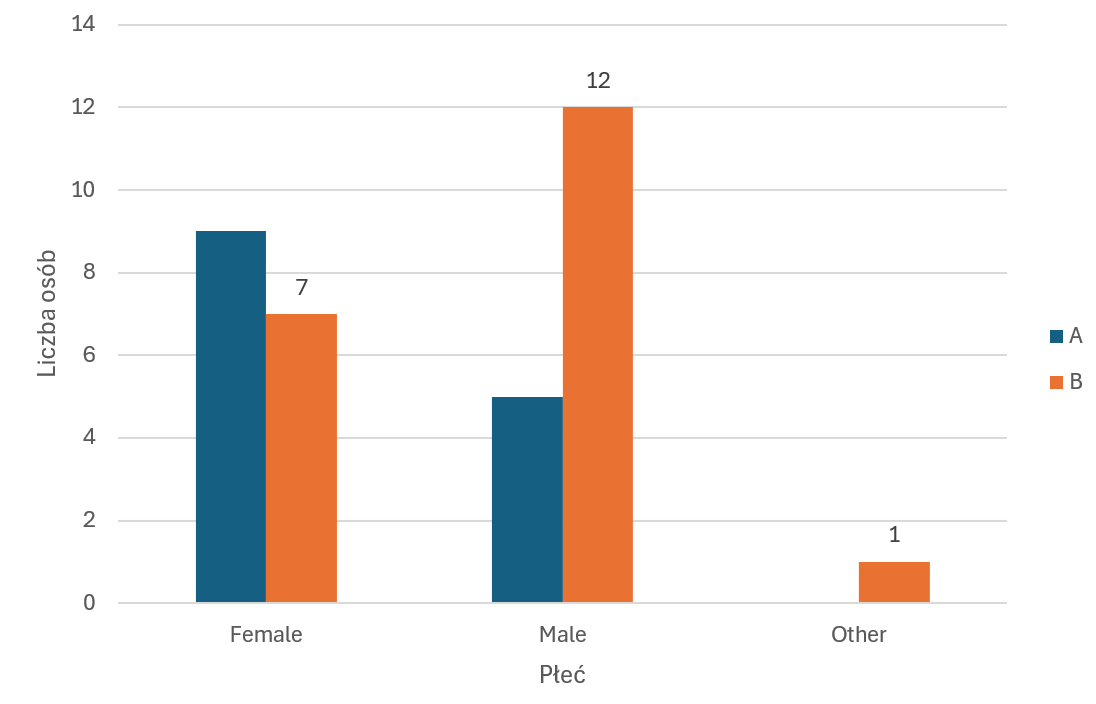
\includegraphics[width=0.9\textwidth]{demo1.png}
    \caption{Płeć uczestników badania z podziałem na formularz A i B}
    \label{fig:ch7_demo1}
\end{figure}

Większość uczestników należała do grupy wiekowej 20-29 lat, co odzwierciedlają dane przedstawione w
tabeli \ref{tab1:ch7_2} i na rysunku \ref{fig:ch7_demo2} . Wśród wypełniających formularz A było 7 osób
w wieku 20-29 lat, a w przypadku formularza B - 11 osób. Uczestnicy reprezentowali jednak różne grupy
wiekowe, od nastolatków po osoby po 30. i 40. roku życia.

\begin{table}[h!]
    \begin{center}
        \begin{tabular}{|l|r|r|}
            \hline
            Przedział wiekowy & Liczba osób & Procent całości \\
            \hline
            15-19             & 4           & 11.76\%         \\
            20-24             & 12          & 35.29\%         \\
            25-29             & 8           & 23.53\%         \\
            30-34             & 6           & 17.65\%         \\
            35-39             & 3           & 8.82\%          \\
            40-45             & 1           & 2.94\%          \\
            \hline
        \end{tabular}
    \end{center}
    \caption{Uczestnicy badania ze względu na wiek}\label{tab1:ch7_2}
\end{table}

\begin{figure}[h!]
    \centering
    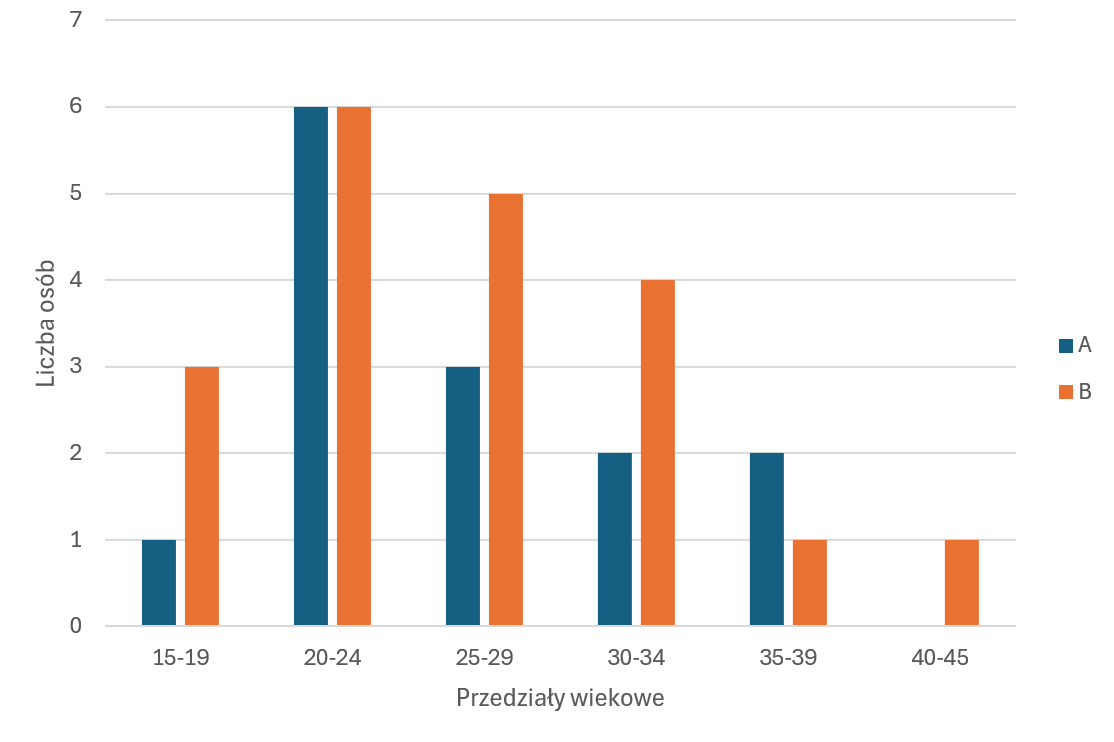
\includegraphics[width=0.9\textwidth]{demo2.png}
    \caption{Wiek uczestników badania z podziałem na formularz A i B}
    \label{fig:ch7_demo2}
\end{figure}

Uczestnicy badania pochodzili z różnych kontynentów, jednak dominowali mieszkańcy Europy i Stanów
Zjednoczonych, co widać wyraźnie na rysunku \ref{fig:ch7_demo3} i w tabeli \ref{tab1:ch7_3} . Najwięcej
osób wypełniających formularz A pochodziło z Polski, Holandii, Rosji i Wielkiej Brytanii. Z kolei w
przypadku formularza B, największe reprezentacje miały Stany Zjednoczone, Wielka Brytania i Niemcy.

\begin{table}[h!]
    \begin{center}
        \begin{tabular}{|l|r|r|}
            \hline
            Kraj pochodzenia  & Liczba osób & Procent całości \\
            \hline
            Antigua i Barbuda & 1           & 2.94\%          \\
            Argentyna         & 1           & 2.94\%          \\
            Chiny             & 1           & 2.94\%          \\
            Filipiny          & 1           & 2.94\%          \\
            Francja           & 3           & 8.82\%          \\
            Holandia          & 2           & 5.88\%          \\
            Indie             & 3           & 8.82\%          \\
            Niemcy            & 3           & 8.82\%          \\
            Nowa Zelandia     & 1           & 2.94\%          \\
            Polska            & 2           & 5.88\%          \\
            Portugalia        & 1           & 2.94\%          \\
            Rosja             & 1           & 2.94\%          \\
            Stany Zjednoczone & 7           & 20.59\%         \\
            Szwecja           & 1           & 2.94\%          \\
            Ukraina           & 1           & 2.94\%          \\
            Wielka Brytania   & 5           & 14.71\%         \\
            \hline
        \end{tabular}
    \end{center}
    \caption{Uczestnicy badania ze względu na kraj pochodzenia}\label{tab1:ch7_3}
\end{table}

\begin{figure}[h!]
    \centering
    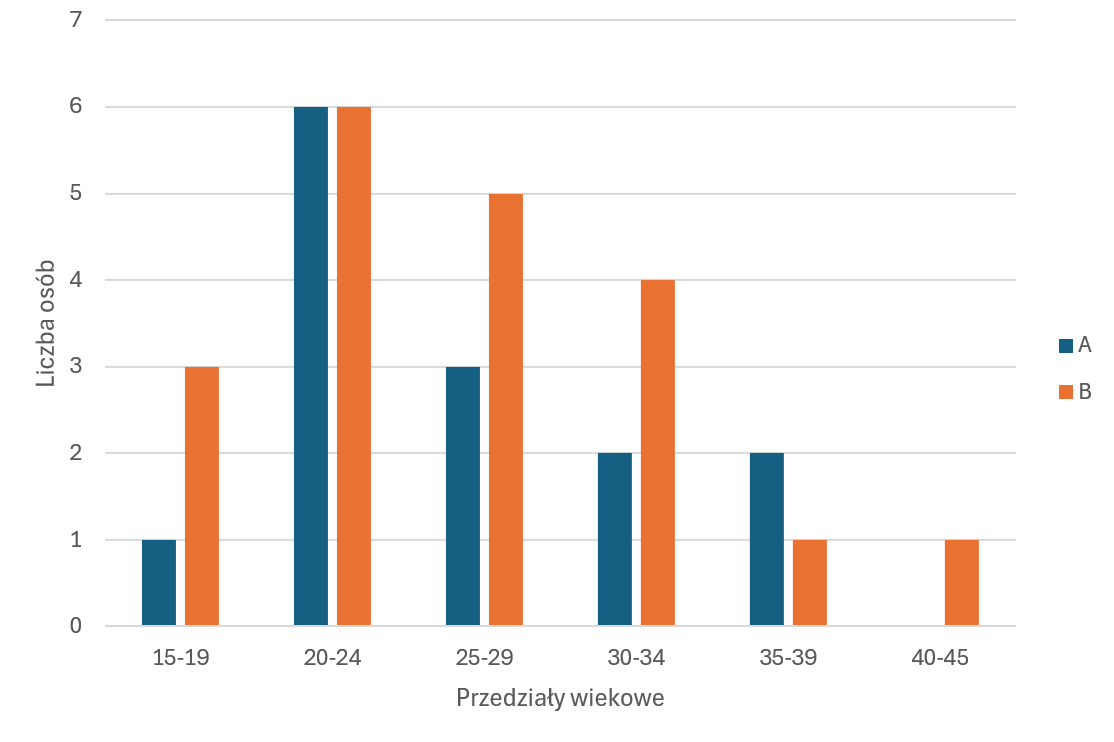
\includegraphics[width=0.9\textwidth]{demo3.png}
    \caption{Kraj pochodzenia uczestników badania z podziałem na formularz A i B}
    \label{fig:ch7_demo3}
\end{figure}

\newpage

Interesującym aspektem badania był wiek, w którym uczestnicy rozpoczęli przygodę z grami wideo. Jak
pokazują dane w tabeli \ref{tab1:ch7_4}  i na rysunku \ref{fig:ch7_demo4} , zdecydowana większość osób
zaczęła grać w wieku 7-12 lat. Tylko nieliczni zadeklarowali, że zaczęli grać przed 7. rokiem życia
lub w okresie nastoletnim (13-19 lat).

\begin{table}[h!]
    \begin{center}
        \begin{tabular}{|l|r|r|}
            \hline
            Wiek rozpoczęcia grania w gry wideo & Liczba osób & Procent całości \\
            \hline
            <7                                  & 7           & 20.59\%         \\
            7-12                                & 19          & 55.88\%         \\
            13-15                               & 5           & 14.71\%         \\
            16-19                               & 2           & 5.88\%          \\
            20+                                 & 1           & 2.94\%          \\
            \hline
        \end{tabular}
    \end{center}
    \caption{Uczestnicy badania ze względu na wiek rozpoczęcia grania w gry wideo}\label{tab1:ch7_4}
\end{table}

\begin{figure}[h!]
    \centering
    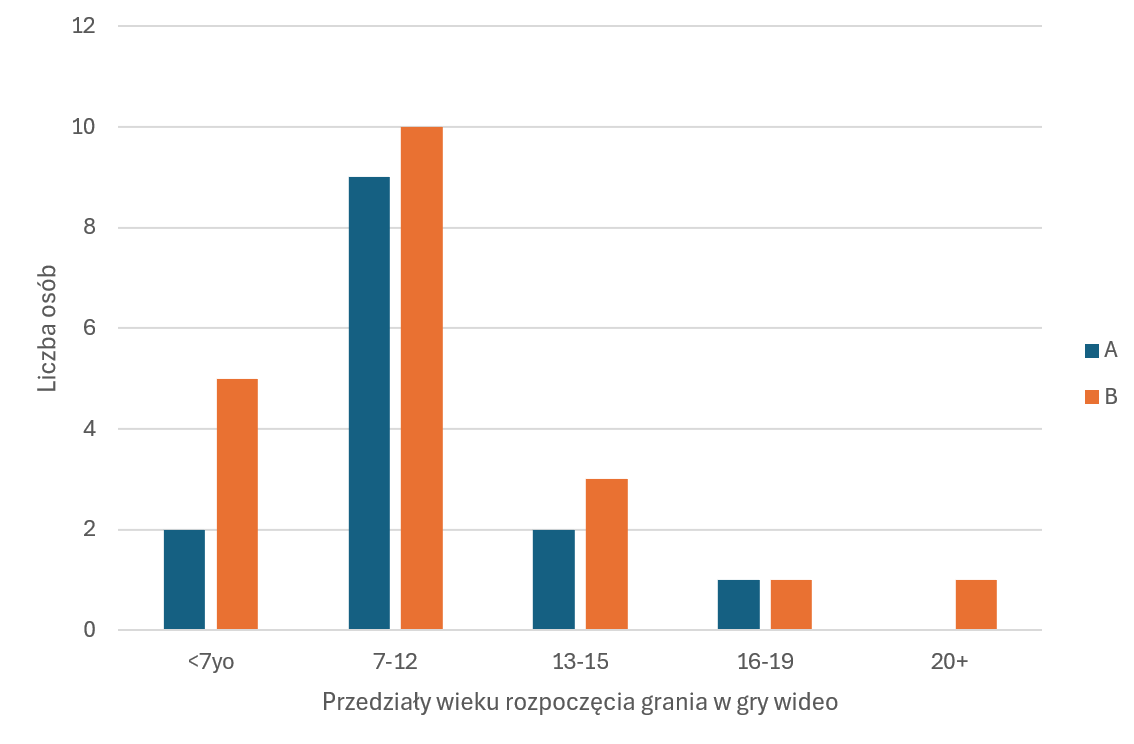
\includegraphics[width=0.9\textwidth]{demo4.png}
    \caption{Wiek rozpoczęcia grania w gry wideo przez uczestników badania z podziałem na formularz A i B}
    \label{fig:ch7_demo4}
\end{figure}

\newpage

Wreszcie, z danych przedstawionych na rysunku \ref{fig:ch7_demo5} i w tabeli \ref{tab1:ch7_5} wynika, że uczestnicy średnio nie spędzali
więcej niż 10 godzin tygodniowo na graniu. Najwięcej osób deklarowało granie przez mniej niż 5 godzin
tygodniowo lub w przedziale 5-10 godzin. Tylko nieliczni przyznali, że grają ponad 20 godzin tygodniowo.

\begin{table}[h!]
    \begin{center}
        \begin{tabular}{|m{15em}|r|r|}
            \hline
            Średnia liczba godzin tygodniowo \newline przeznaczona na gry wideo & Liczba osób & Procent całości \\
            \hline
            <5h                                                                 & 16          & 47.06\%         \\
            5-10h                                                               & 10          & 29.41\%         \\
            10-15h                                                              & 2           & 5.88\%          \\
            15-20h                                                              & 2           & 5.88\%          \\
            >20h                                                                & 4           & 11.76\%         \\
            \hline
        \end{tabular}
    \end{center}
    \caption{Uczestnicy badania ze względu na średnią liczbę godzin tygodniowo przeznaczonych na gry wideo}\label{tab1:ch7_5}
\end{table}

\begin{figure}[h!]
    \centering
    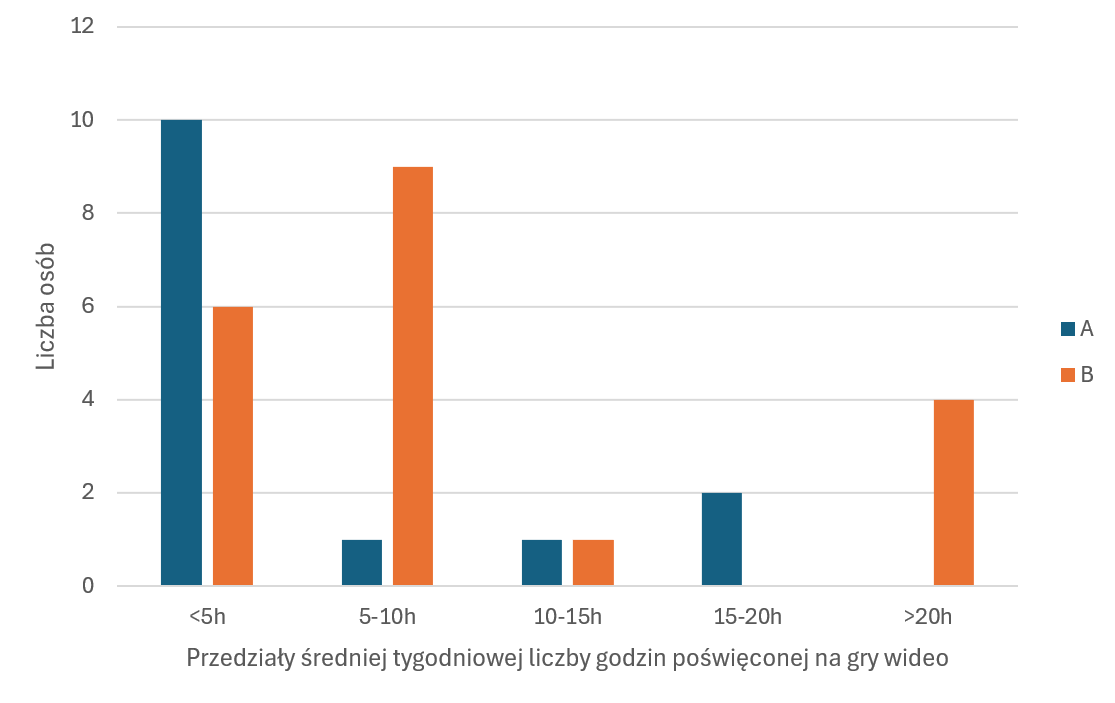
\includegraphics[width=0.9\textwidth]{demo5.png}
    \caption{Średnia liczba godzin tygodniowo przeznaczona na gry wideo przez uczestników badania z podziałem na formularz A i B}
    \label{fig:ch7_demo5}
\end{figure}

\section{Analiza danych}\label{section:ch7_2}

Tutaj będzie tekst bla bla bla

\begin{table}[h!]
    \begin{center}
        \begin{tabular}{|m{10em}|m{5em}|m{5em}|m{5em}|m{5em}|}
            \hline
            Pytanie                                                                     & Wartość statystyki (non-AI) & P-value (non-AI) & Wartość statystyki (AI) & P-value (AI)   \\
            \hline
            1. Tracę poczucie czasu                                                     & 0.911                       & 0.164            & 0.900                   & 0.113          \\
            2. Byłem/-am \newline zainteresowany/-a fabułą gry                          & 0.923                       & 0.243            & 0.881                   & 0.060          \\
            3. Czuję się inaczej\textbf{*}                                              & 0.855                       & \textbf{0.026}   & 0.886                   & 0.070          \\
            4. Czułem/-am, że mogę odkrywać różne rzeczy\textbf{*}                      & 0.755                       & \textbf{0.001}   & 0.837                   & \textbf{0.015} \\
            5. Gra wydaje się prawdziwa\textbf{*}                                       & 0.841                       & \textbf{0.017}   & 0.903                   & 0.127          \\
            6. Byłem/-am \newline w pełni zajęty/-a grą\textbf{*}                       & 0.850                       & \textbf{0.023}   & 0.896                   & 0.100          \\
            7. Denerwuję się\textbf{*}                                                  & 0.900                       & 0.111            & 0.814                   & \textbf{0.007} \\
            8. Czas jakby stanął w miejscu lub się zatrzymał\textbf{*}                  & 0.834                       & \textbf{0.013}   & 0.837                   & \textbf{0.015} \\
            9. Czuję się \newline rozkojarzony/-a\textbf{*}                             & 0.864                       & \textbf{0.034}   & 0.814                   & \textbf{0.007} \\
            10. Byłem/-am głęboko \newline skoncentrowany/-a \newline na grze\textbf{*} & 0.914                       & 0.181            & 0.848                   & \textbf{0.021} \\
            11. Zmęczyłem/-am się\textbf{*}                                             & 0.867                       & \textbf{0.038}   & 0.909                   & 0.152          \\
            12. Granie wydaje się automatyczne\textbf{*}                                & 0.924                       & 0.253            & 0.842                   & \textbf{0.017} \\
            13. Moje myśli \newline biegną szybko\textbf{*}                             & 0.932                       & 0.326            & 0.836                   & \textbf{0.014} \\
            14. Podobało mi się\textbf{*}                                               & 0.878                       & 0.054            & 0.875                   & \textbf{0.049} \\
            15. Gram bez zastanawiania się jak grać\textbf{*}                           & 0.805                       & \textbf{0.006}   & 0.896                   & 0.100          \\
            16. Granie sprawia, \newline że czuję się spokojny/-a\textbf{*}             & 0.911                       & 0.164            & 0.844                   & \textbf{0.018} \\
            17. Gram dłużej \newline niż zamierzałem/-am\textbf{*}                      & 0.820                       & \textbf{0.009}   & 0.855                   & \textbf{0.026} \\
            18. Naprawdę wczuwam się w grę                                              & 0.923                       & 0.246            & 0.885                   & 0.069          \\
            19. Czuję, że nie mogę przestać grać\textbf{*}                              & 0.786                       & \textbf{0.003}   & 0.744                   & \textbf{0.001} \\
            \hline
        \end{tabular}
    \end{center}
    \caption{Wyniki testu Shapiro-Wilka dla formularza A i obu wersji gier}\label{tab1:ch7_10}
\end{table}

\begin{table}[h!]
    \begin{center}
        \begin{tabular}{|m{10em}|m{5em}|m{5em}|m{5em}|m{5em}|}
            \hline
            Pytanie                                                                     & Wartość statystyki (non-AI) & P-value (non-AI) & Wartość statystyki (AI) & P-value (AI)   \\
            \hline
            1. Tracę poczucie czasu\textbf{*}                                           & 0.892                       & \textbf{0.029}   & 0.836                   & \textbf{0.003} \\
            2. Byłem/-am \newline zainteresowany/-a fabułą gry\textbf{*}                & 0.875                       & \textbf{0.014}   & 0.864                   & \textbf{0.009} \\
            3. Czuję się inaczej\textbf{*}                                              & 0.793                       & \textbf{0.001}   & 0.882                   & \textbf{0.019} \\
            4. Czułem/-am, że mogę odkrywać różne rzeczy\textbf{*}                      & 0.856                       & \textbf{0.007}   & 0.728                   & \textbf{0.000} \\
            5. Gra wydaje się prawdziwa\textbf{*}                                       & 0.827                       & \textbf{0.002}   & 0.867                   & \textbf{0.010} \\
            6. Byłem/-am \newline w pełni zajęty/-a grą\textbf{*}                       & 0.854                       & \textbf{0.006}   & 0.842                   & \textbf{0.004} \\
            7. Denerwuję się\textbf{*}                                                  & 0.792                       & \textbf{0.001}   & 0.847                   & \textbf{0.005} \\
            8. Czas jakby stanął w miejscu lub się zatrzymał\textbf{*}                  & 0.827                       & \textbf{0.002}   & 0.864                   & \textbf{0.009} \\
            9. Czuję się \newline rozkojarzony/-a\textbf{*}                             & 0.865                       & \textbf{0.010}   & 0.917                   & \textbf{0.088} \\
            10. Byłem/-am głęboko \newline skoncentrowany/-a \newline na grze\textbf{*} & 0.883                       & \textbf{0.020}   & 0.792                   & \textbf{0.001} \\
            11. Zmęczyłem/-am się\textbf{*}                                             & 0.860                       & \textbf{0.008}   & 0.902                   & \textbf{0.045} \\
            12. Granie wydaje się automatyczne\textbf{*}                                & 0.789                       & \textbf{0.001}   & 0.893                   & \textbf{0.031} \\
            14. Podobało mi się\textbf{*}                                               & 0.890                       & \textbf{0.000}   & 0.865                   & \textbf{0.010} \\
            15. Gram bez zastanawiania się jak grać\textbf{*}                           & 0.746                       & \textbf{0.006}   & 0.896                   & \textbf{0.034} \\
            16. Granie sprawia, \newline że czuję się spokojny/-a\textbf{*}             & 0.851                       & \textbf{0.006}   & 0.825                   & \textbf{0.002} \\
            17. Gram dłużej \newline niż zamierzałem/-am\textbf{*}                      & 0.840                       & \textbf{0.004}   & 0.860                   & \textbf{0.008} \\
            18. Naprawdę wczuwam się w grę\textbf{*}                                    & 0.876                       & \textbf{0.015}   & 0.875                   & \textbf{0.015} \\
            19. Czuję, że nie mogę przestać grać\textbf{*}                              & 0.850                       & \textbf{0.005}   & 0.882                   & \textbf{0.019} \\
            \hline
        \end{tabular}
    \end{center}
    \caption{Wyniki testu Shapiro-Wilka dla formularza B i obu wersji gier}\label{tab1:ch7_11}
\end{table}

\begin{table}[h!]
    \begin{center}
        \begin{tabular}{|m{10em}|m{5em}|m{5em}|m{5em}|m{5em}|}
            \hline
            Pytanie                                                           & Wartość statystyki (non-AI) & P-value (non-AI) & Wartość statystyki (AI) & P-value (AI) \\
            \hline
            1. Tracę poczucie czasu                                           & 0.613                       & 0.439            & 0.313                   & 0.580        \\
            2. Byłem/-am \newline zainteresowany/-a fabułą gry                & 0.121                       & 0.730            & 1.395                   & 0.246        \\
            3. Czuję się inaczej                                              & 1.202                       & 0.281            & 0.141                   & 0.710        \\
            4. Czułem/-am, że mogę odkrywać różne rzeczy                      & 3.149                       & 0.086            & 0.004                   & 0.949        \\
            5. Gra wydaje się prawdziwa                                       & 2.329                       & 0.137            & 0.054                   & 0.818        \\
            6. Byłem/-am \newline w pełni zajęty/-a grą                       & 0.070                       & 0.793            & 0.281                   & 0.600        \\
            7. Denerwuję się                                                  & 0.388                       & 0.538            & 0.168                   & 0.685        \\
            8. Czas jakby stanął w miejscu lub się zatrzymał                  & 1.340                       & 0.256            & 0.121                   & 0.731        \\
            9. Czuję się \newline rozkojarzony/-a                             & 0.980                       & 0.330            & 0.000                   & 1.000        \\
            10. Byłem/-am głęboko \newline skoncentrowany/-a \newline na grze & 0.009                       & 0.926            & 1.252                   & 0.272        \\
            11. Zmęczyłem/-am się                                             & 0.003                       & 0.956            & 0.059                   & 0.810        \\
            12. Granie wydaje się automatyczne                                & 0.408                       & 0.528            & 2.819                   & 0.103        \\
            13. Moje myśli \newline biegną szybko                             & 0.693                       & 0.411            & 0.604                   & 0.443        \\
            14. Podobało mi się                                               & 0.163                       & 0.689            & 2.875                   & 0.100        \\
            15. Gram bez zastanawiania się jak grać                           & 1.740                       & 0.196            & 0.227                   & 0.637        \\
            16. Granie sprawia, \newline że czuję się spokojny/-a             & 0.000                       & 1.000            & 1.026                   & 0.319        \\
            17. Gram dłużej \newline niż zamierzałem/-am                      & 1.355                       & 0.253            & 0.320                   & 0.576        \\
            18. Naprawdę wczuwam się w grę                                    & 0.254                       & 0.617            & 0.399                   & 0.532        \\
            19. Czuję, że nie mogę przestać grać                              & 0.508                       & 0.481            & 0.640                   & 0.430        \\
            \hline
        \end{tabular}
    \end{center}
    \caption{Wyniki testu Levene'a porównującego wariancję pomiędzy formularzem A i B odpowiednio dla wersji gier bez AI i z AI}\label{tab1:ch7_12}
\end{table}

% TODO: Wilcoxon i Mann-Whitney jako 2 tabelki (też scalić)
% no i Kruskal-Wallis też scalony w jedną będzie, w sumie 3 tabelki jak wyżej i finito

\begin{table}[h!]
    \begin{center}
        \begin{tabular}{|m{10em}|m{5em}|m{5em}|m{5em}|m{5em}|}
            \hline
            Pytanie                                                           & Wartość statystyki (A) & P-value (A)    & Wartość statystyki (B) & P-value (B)    \\
            \hline
            1. Tracę poczucie czasu                                           & 8                      & 0.132          & 12.5                   & 0.061          \\
            2. Byłem/-am \newline zainteresowany/-a fabułą gry                & 6                      & 0.679          & 27.5                   & 0.184          \\
            3. Czuję się inaczej                                              & 4                      & 0.334          & 21                     & 0.499          \\
            4. Czułem/-am, że mogę odkrywać różne rzeczy\textbf{*}            & 1.5                    & \textbf{0.003} & 0                      & \textbf{0.002} \\
            5. Gra wydaje się prawdziwa\textbf{*}                             & 0                      & \textbf{0.010} & 19.5                   & 0.713          \\
            6. Byłem/-am \newline w pełni zajęty/-a grą                       & 6.5                    & 0.783          & 41.5                   & 0.775          \\
            7. Denerwuję się                                                  & 10.5                   & 0.546          & 7                      & 0.058          \\
            8. Czas jakby stanął w miejscu lub się zatrzymał                  & 11                     & 0.603          & 25                     & 0.249          \\
            9. Czuję się \newline rozkojarzony/-a                             & 1.5                    & 0.414          & 22.5                   & 0.179          \\
            10. Byłem/-am głęboko \newline skoncentrowany/-a \newline na grze & 6.5                    & 0.783          & 22.5                   & 0.599          \\
            11. Zmęczyłem/-am się                                             & 18                     & 0.582          & 28                     & 0.651          \\
            12. Granie wydaje się automatyczne\textbf{*}                      & 1                      & \textbf{0.025} & 5                      & \textbf{0.021} \\
            13. Moje myśli \newline biegną szybko                             & 0                      & 0.059          & 20                     & 0.405          \\
            14. Podobało mi się                                               & 9                      & 0.748          & 20                     & 0.218          \\
            15. Gram bez zastanawiania się jak grać\textbf{*}                 & 5                      & 0.066          & 3                      & \textbf{0.007} \\
            16. Granie sprawia, \newline że czuję się spokojny/-a             & 14.5                   & 0.618          & 34.5                   & 0.714          \\
            17. Gram dłużej \newline niż zamierzałem/-am\textbf{*}            & 6                      & 0.655          & 6                      & \textbf{0.026} \\
            18. Naprawdę wczuwam się w grę                                    & 10.5                   & 1.000          & 16                     & 0.222          \\
            19. Czuję, że nie mogę przestać grać                              & 2                      & 0.564          & 21                     & 0.490          \\
            \hline
        \end{tabular}
    \end{center}
    \caption{Wyniki testu Wilcoxona porównującego zmianę ocen pytań wewnątrz formularza A i B}\label{tab1:ch7_13}
\end{table}

\begin{table}[h!]
    \begin{center}
        \begin{tabular}{|m{10em}|m{5em}|m{5em}|m{5em}|m{5em}|}
            \hline
            Pytanie                                                           & Wartość statystyki (non-AI) & P-value (non-AI) & Wartość statystyki (AI) & P-value (AI)   \\
            \hline
            1. Tracę poczucie czasu\textbf{*}                                 & 133                         & 0.816            & 77                      & \textbf{0.025} \\
            2. Byłem/-am \newline zainteresowany/-a fabułą gry                & 118                         & 0.440            & 100                     & 0.154          \\
            3. Czuję się inaczej                                              & 121                         & 0.503            & 123.5                   & 0.567          \\
            4. Czułem/-am, że mogę odkrywać różne rzeczy\textbf{*}            & 58.5                        & \textbf{0.004}   & 221                     & \textbf{0.004} \\
            5. Gra wydaje się prawdziwa\textbf{*}                             & 77                          & \textbf{0.023}   & 133.5                   & 0.829          \\
            6. Byłem/-am \newline w pełni zajęty/-a grą                       & 112                         & 0.323            & 101                     & 0.167          \\
            7. Denerwuję się                                                  & 154.5                       & 0.611            & 138.5                   & 0.971          \\
            8. Czas jakby stanął w miejscu lub się zatrzymał                  & 106                         & 0.227            & 95                      & 0.110          \\
            9. Czuję się \newline rozkojarzony/-a                             & 115.5                       & 0.389            & 85                      & 0.051          \\
            10. Byłem/-am głęboko \newline skoncentrowany/-a \newline na grze & 106.5                       & 0.237            & 107                     & 0.242          \\
            11. Zmęczyłem/-am się                                             & 133.5                       & 0.829            & 159                     & 0.504          \\
            12. Granie wydaje się automatyczne\textbf{*}                      & 84.5                        & \textbf{0.044}   & 88                      & 0.064          \\
            13. Moje myśli \newline biegną szybko                             & 120.5                       & 0.493            & 92.5                    & 0.090          \\
            14. Podobało mi się                                               & 123                         & 0.552            & 106                     & 0.221          \\
            15. Gram bez zastanawiania się jak grać                           & 107                         & 0.220            & 113.5                   & 0.352          \\
            16. Granie sprawia, \newline że czuję się spokojny/-a\textbf{*}   & 97.5                        & 0.129            & 72.5                    & \textbf{0.015} \\
            17. Gram dłużej \newline niż zamierzałem/-am\textbf{*}            & 129.5                       & 0.719            & 84.5                    & \textbf{0.048} \\
            18. Naprawdę wczuwam się w grę                                    & 119.5                       & 0.474            & 105.5                   & 0.222          \\
            19. Czuję, że nie mogę przestać grać                              & 102                         & 0.175            & 87.5                    & 0.062          \\
            \hline
        \end{tabular}
    \end{center}
    \caption{Wyniki testu Manna-Whitneya porównującego skalę ocen wersji gier bez AI i z AI pomiędzy formularzem A i B}\label{tab1:ch7_14}
\end{table}

Pojawi się jeszcze analiza jakościowa odnośnie pytań otwartych poniżej: